\documentclass[fleqn]{article}
\usepackage[margin=1in]{geometry}
\usepackage[nodisplayskipstretch]{setspace}
\usepackage{amsmath, nccmath, bm}
\usepackage{amssymb}
\usepackage{enumitem}
\usepackage{graphicx}
\usepackage{float}
\usepackage{listings}
\usepackage{hyperref}
\usepackage[svgnames]{xcolor}
\graphicspath{{./images}}

\hypersetup{
    colorlinks=true,
    linkcolor=black,
    filecolor=black,      
    urlcolor=blue
    }

\newcommand{\zerodisplayskip}{
	\setlength{\abovedisplayskip}{0pt}%
	\setlength{\belowdisplayskip}{0pt}%
	\setlength{\abovedisplayshortskip}{0pt}%
	\setlength{\belowdisplayshortskip}{0pt}%
	\setlength{\mathindent}{0pt}}
	
\definecolor{vgreen}{RGB}{104,180,104}
\definecolor{vblue}{RGB}{49,49,255}
\definecolor{vorange}{RGB}{255,143,102}

\lstdefinestyle{verilog-style}
{
    language=Verilog,
    basicstyle=\small\ttfamily,
    keywordstyle=\color{vblue},
    identifierstyle=\color{black},
    commentstyle=\color{vgreen},
    numbers=left,
    numberstyle=\tiny\color{black},
    numbersep=10pt,
    tabsize=8,
    moredelim=*[s][\colorIndex]{[}{]},
    literate=*{:}{:}1
}

\lstset{style={verilog-style},showstringspaces=false}

\makeatletter
\newcommand*\@lbracket{[}
\newcommand*\@rbracket{]}
\newcommand*\@colon{:}
\newcommand*\colorIndex{%
    \edef\@temp{\the\lst@token}%
    \ifx\@temp\@lbracket \color{black}%
    \else\ifx\@temp\@rbracket \color{black}%
    \else\ifx\@temp\@colon \color{black}%
    \else \color{vorange}%
    \fi\fi\fi
}
\makeatother

\newcommand{\code}[1]{%
	\colorbox{Gainsboro}{\texttt{#1}}%
}

\title{Homework 2}
\author{Owen Sowatzke}
\date{February 24, 2025}

\begin{document}

	\offinterlineskip
	\setlength{\lineskip}{12pt}
	\zerodisplayskip
	\maketitle
	
	\begin{enumerate}
		\item Based on the figures below mention which figure depicts the mode of operation and briefly describe its operation in terms of the figure.
		
		\begin{enumerate}
		
			\item Figure \ref{fig::mode_of_operations_part_a} depicts the subthreshold region.
			
			\begin{figure}[H]				
				\centerline{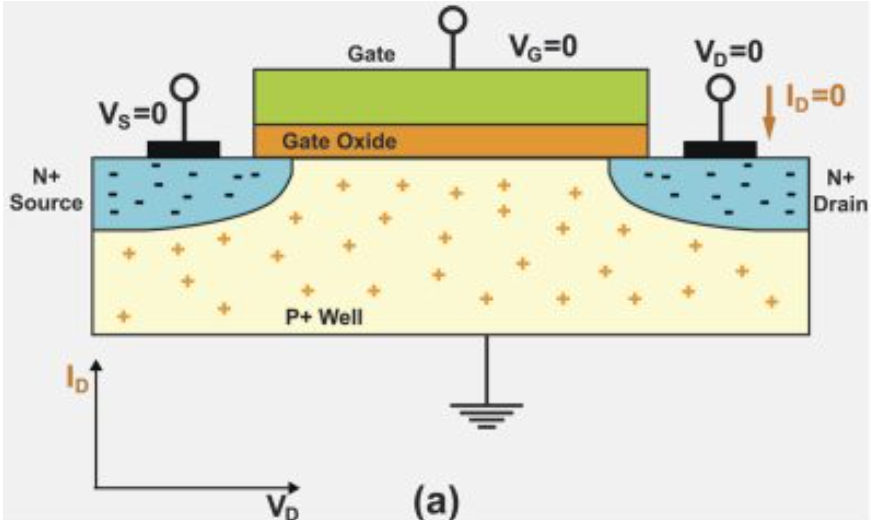
\includegraphics[width=0.5\textwidth]{mode_of_operations_part_a.png}}
				\caption{CMOS Transistor in Subthreshold Region}
				\label{fig::mode_of_operations_part_a}
			\end{figure}
		
			\item Figure \ref{fig::mode_of_operations_part_b} depicts the resistive region.
			
			\begin{figure}[H]				
				\centerline{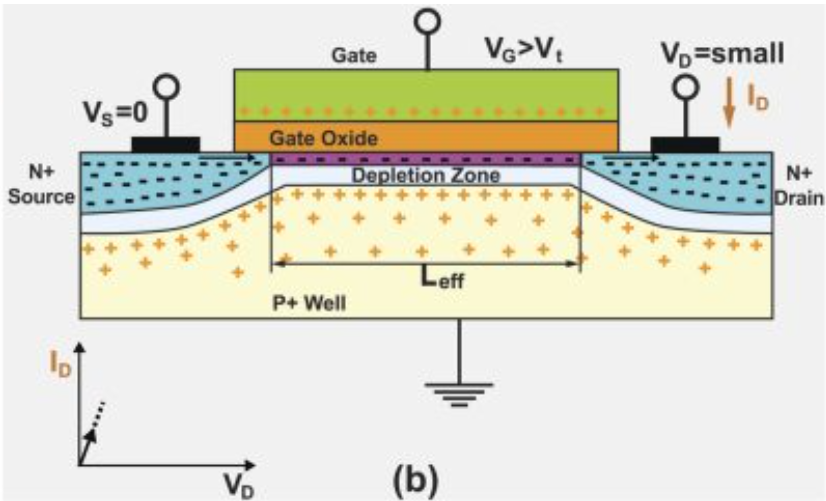
\includegraphics[width=0.5\textwidth]{mode_of_operations_part_b.png}}
				\caption{CMOS Transistor in Resistive Region}
				\label{fig::mode_of_operations_part_b}
			\end{figure}
			
			\item Figure \ref{fig::mode_of_operations_part_c} depicts the start of the saturation region.
			
			\begin{figure}[H]				
				\centerline{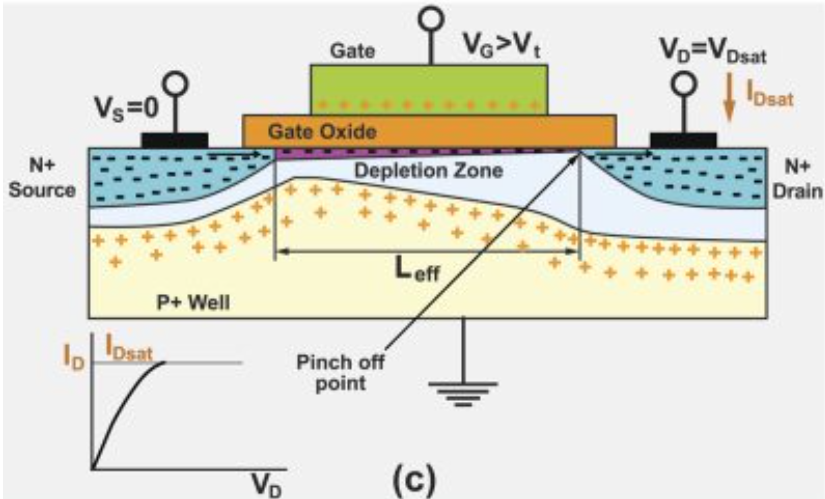
\includegraphics[width=0.5\textwidth]{mode_of_operations_part_c.png}}
				\caption{CMOS Transistor on Boundary of Saturation Region}
				\label{fig::mode_of_operations_part_c}
			\end{figure}
		
			\item Figure \ref{fig::mode_of_operations_part_d} depicts the saturation region.
			
			\begin{figure}[H]				
				\centerline{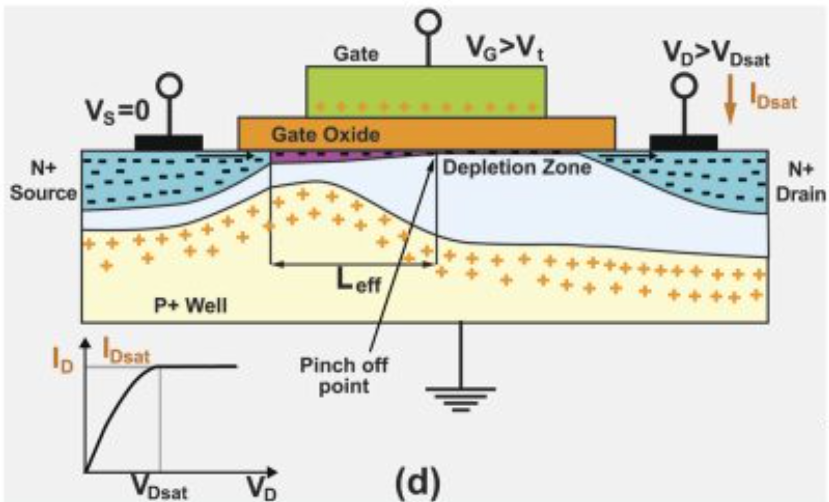
\includegraphics[width=0.5\textwidth]{mode_of_operations_part_d.png}}
				\caption{CMOS Transistor in Saturation Region}
				\label{fig::mode_of_operations_part_d}
			\end{figure}
			
		\end{enumerate}
		
	\end{enumerate}

\end{document}